
\subsection{Observed and predicted event yields}
\label{sec:cutflow}

Table~\ref{tab:CFComp} compares the event yields after applying the analysis cuts with data and the 2 MC samples for each year, and table~\ref{tab:RelCF} shows a relative comparison between the cuts.  Note that the event selection has been validated using an independent implementation of the analysis event selection using the $ZH\rightarrow aa\rightarrow gggg$ analysis framework\footnote{We thank Murtaza Safdari for helping with this.  The analysis code is built on the BHamAnalyaisFramework: \url{https://gitlab.cern.ch/atlas-physics/HDBS/HBSM/higgs_axion_axion/-/tree/workingCompile/BhamAnalysisFramework}.}.

\begin{table}[h!]
    \centering
    \begin{tabular}{l|l|l|l|l|l|l}
    \hline\hline
    \textbf{Sample} & \multicolumn{6}{c}{\textbf{Cuts}} \\ \hline
     & None & DQ & Trigger & Dilepton & $p_{\text{T},\ell\ell}$ & $p_{\text{T},\ell\ell}$ \\
     &  &  &  &  & $>165~\GeV$ & $>200~\GeV$ \\ \hline\hline
    Data 2015-2016 & 475.7M & 462.5M & 72.89M & 20.27M & 103.5k & 54.92k \\ \hline
    Powheg Pythia 8 MC16a & 70.63M & 70.28M & 41.27M & 20.11M & 79.31k & 41.15k \\ \hline
    Sherpa 2.2.1 MC16a & 75.60M & 75.21M & 42.28M & 20.06M & 96.72k & 52.03k \\ \hline\hline
    Data 2017 & 282.8M & 270.5M & 84.38M & 24.15M & 124.2k & 65.87k \\ \hline
    Powheg Pythia 8 MC16d & 86.42M & 85.88M & 50.35M & 24.45M & 96.58k & 50.08k \\ \hline
    Sherpa 2.2.1 MC16d & 92.50M & 91.90M & 51.59M & 24.41M & 118.3k & 63.30k \\ \hline\hline
    Data 2018 & 357.0M & 348.7M & 116.8M & 35.99M & 163.4k & 86.35k \\ \hline
    Powheg Pythia 8 MC16e & 114.0M & 113.3M & 67.22M & 32.46M & 128.2k & 66.56k \\ \hline
    Sherpa 2.2.1 MC16e & 122.0M & 121.3M & 68.93M & 36.41M & 155.9k & 83.23k \\ \hline\hline
    \end{tabular}
    \caption{Number of events remaining after each cut applied during the analysis. Data Quality (DQ) includes the GRL and event cleaning criteria.
    Dilepton includes the checks for 2 oppositely charged muons which pass TTVA and trigger matching requirements, as well as the $m_{\ell\ell}$ cut.
    Differences between MC and data are expected up to the dilepton cut as data contains QCD background while the MC samples do not.}
    \label{tab:CFComp}
\end{table}

\begin{table}[h!]
  \centering
  \begin{tabular}{l|l|l|l|l|l}
  \hline\hline
  \textbf{Sample} & \multicolumn{5}{c}{\textbf{Cuts}} \\ \hline
    & DQ & Trigger & Dilepton & $p_{\text{T},\ell\ell}$ & $p_{\text{T},\ell\ell}$ \\
    &  &  &  & $>165~\GeV$ & $>200~\GeV$ \\ \hline\hline
   Data 2015-2016 & -2.46\% & -84.24\% & -72.20\% & -99.49\% & -46.93\% \\ \hline
   Powheg Pythia 8 MC16a & -0.50\% & -41.27\% & -51.27\% & -99.61\% & -48.11\% \\ \hline
   Sherpa 2.2.1 MC16a & -0.50\% & -43.78\% & -52.56\% & -99.52\% & -46.21\% \\ \hline\hline
   Data 2017 & -4.35\% & -68.61\% & -71.38\% & -99.49\% & -46.93\% \\ \hline
   Powheg Pythia 8 MC16d & -0.63\% & -41.37\% & -51.45\% & -99.60\% & -48.15\% \\ \hline
   Sherpa 2.2.1 MC16d & -0.64\% & -43.87\% & -52.68\% & -99.52\% & -46.51\% \\ \hline\hline
   Data 2018 & -2.30\% & -66.50\% & -72.88\% & -99.48\% & -47.04\% \\ \hline
   Powheg Pythia 8 MC16e & -0.60\% & -40.69\% & -51.70\% & -99.61\% & -48.97\% \\ \hline
   Sherpa 2.2.1 MC16e & -0.60\% & -43.17\% & -52.95\% & -99.52\% & -46.63\% \\ \hline\hline
   \end{tabular}
   \caption{The relative number of events rejected after each cut compared to the previous cut}
   \label{tab:RelCF}
\end{table}

\subsection{Data stability tests}
\label{sec:data-stability}
To check stability of data used for this analysis, rate for each year is calculated by dividing event counts from a set of runs by their associated total integrated luminosity. Events are counted if they pass the event selection with $p_{\text{T},\ell\ell}>165$ GeV. Consecutive runs are combined until the integrated luminosity amount to at least 2 fb$^{-1}$. Figure~\ref{fig:DataStability} depicts the rate for year 2015 to 2018, where each time-ordered data bin contains data 2 fb$^{-1}$ luminosity. The first bin shows rate for year 2015, bins 2--16 are for year 2016, bins 17--37 and 38--64 represent rate for year 2017 and 2018 respectively. Further, to consider those residual runs having combined luminosities smaller than 2 fb$^{-1}$, the last bin for each year is merged with the previous bin. The calculated average rate for year 2015--2018 is 2812 $\pm$ 4 and shows reasonable consistency for each year. Figure~\ref{fig:DataStability} shows the stability of data for each year used in this analysis.
\begin{figure}[h!]
  \centering
  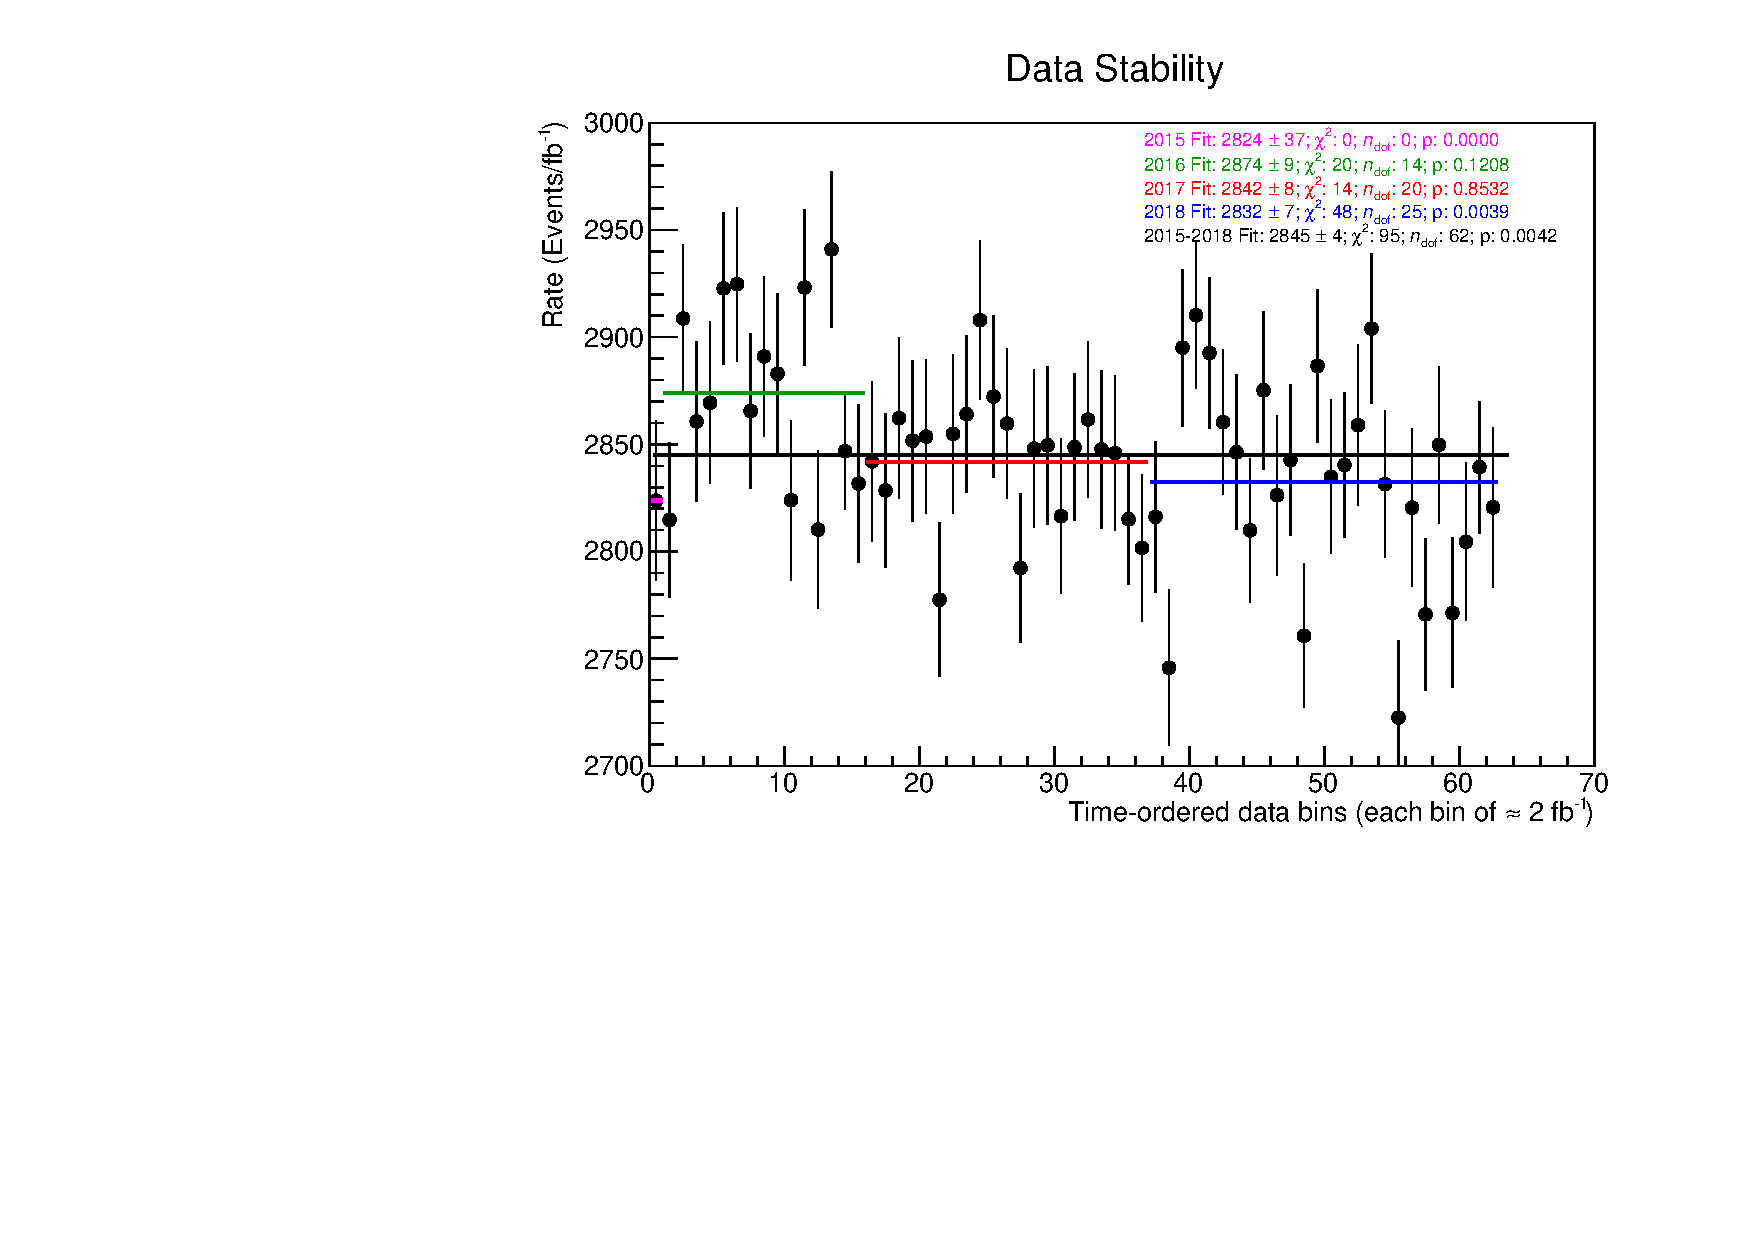
\includegraphics[width=0.75\textwidth]{figures/DataStability.pdf}
  \caption{Events per fb$^{-1}$ for year 2015 to 2018, where each time-ordered data bin contains 2 fb$^{-1}$ luminosity.
    $p$-values and chi-squared values are calculated using statistical uncertainty only. Additional bias is expected due to the changing beam conditions (more or less pileup, affecting e.g.\ lepton isolation).
  }
  \label{fig:DataStability}
\end{figure}

\subsection{Observed and predicted kinematic distributions}
\label{sec:datamc}
Figure~\ref{fig:MuActual} shows the actual interactions per bunch crossing $\mu$ for the individual data periods, as well as the full Run 2 dataset.
Figure~\ref{fig:pTmll} gives the $\pt$ and $m$ distributions for the dilepton system, and figure~\ref{fig:pTetamus} gives the $\pt$ and $\eta$ distributions for both the leading and sub-leading muon.
The $\pt$ and $y$ distributions for the leading and sub-leading track jet are shown in figure~\ref{fig:pTyjets}, and figure~\ref{fig:jetsubstructure} and~\ref{fig:ntrackinjets} show some
selected jet substructure variables and the number of constituents, respectively. Finally, the properties of the tracks used for the analysis are shown in figure~\ref{fig:trackInfo}.


\begin{figure}[h!]
  \centering
  \includegraphics[page=5,width=0.45\textwidth]{figures/ZjetOmnifoldMCDataComp.pdf}
  \includegraphics[page=6,width=0.45\textwidth]{figures/ZjetOmnifoldMCDataComp.pdf} \\
  \includegraphics[page=7,width=0.45\textwidth]{figures/ZjetOmnifoldMCDataComp.pdf}
  \includegraphics[page=8,width=0.45\textwidth]{figures/ZjetOmnifoldMCDataComp.pdf}
  \caption{The ``actual'' mean interactions per bunch crossing, $\mu$, for 2015--2016 data (top left), 2017 data (top right), 2018 data (bottom left), and the full Run-2 dataset (bottom right). Note that the pileup-reweighing uses actual $\mu$ for 2017 and 2018 data, while $\mu_\mathrm{avg}$, i.e.\ $\mu$ calculated by averaging the actual $\mu$ of all bunches, were used for 2015--2016 data. Hence a worse agreement is seen for this period.}
  \label{fig:MuActual}
\end{figure}

\begin{figure}[h!]
  \centering
  \includegraphics[page=12,width=0.45\textwidth]{figures/ZjetOmnifoldMCDataComp.pdf}
  \includegraphics[page=16,width=0.45\textwidth]{figures/ZjetOmnifoldMCDataComp.pdf}
  \caption{Distributions for the $\pt$ and $m$ of the dilepton system. Due to the high $\pt$ phase space, it is expected that the MC simulation will underpredict the data.}
  \label{fig:pTmll}
\end{figure}

\begin{figure}[h!]
  \centering
  \subfloat[Leading muon]{\includegraphics[page=24,width=0.45\textwidth]{figures/ZjetOmnifoldMCDataComp.pdf}\includegraphics[page=32,width=0.45\textwidth]{figures/ZjetOmnifoldMCDataComp.pdf}} \\
  \subfloat[Sub-leading muon]{\includegraphics[page=28,width=0.45\textwidth]{figures/ZjetOmnifoldMCDataComp.pdf}\includegraphics[page=36,width=0.45\textwidth]{figures/ZjetOmnifoldMCDataComp.pdf}}
  \caption{The $\pt$ and $\eta$ distributions for the (a) leading and (b) the sub-leading muon}
  \label{fig:pTetamus}
\end{figure}

\begin{figure}[h!]
  \centering
  \subfloat[Leading track jet]{\includegraphics[page=72,width=0.45\textwidth]{figures/ZjetOmnifoldMCDataComp.pdf}\includegraphics[page=76,width=0.45\textwidth]{figures/ZjetOmnifoldMCDataComp.pdf}} \\
  \subfloat[Sub-leading track jet]{\includegraphics[page=88,width=0.45\textwidth]{figures/ZjetOmnifoldMCDataComp.pdf}\includegraphics[page=92,width=0.45\textwidth]{figures/ZjetOmnifoldMCDataComp.pdf}}
  \caption{The $\pt$ and $y$ distributions for the (a) leading and (b) the sub-leading jet}
  \label{fig:pTyjets}
\end{figure}

\begin{figure}[h!]
  \centering
  \includegraphics[page=84,width=0.45\textwidth]{figures/ZjetOmnifoldMCDataComp.pdf}
  \includegraphics[page=100,width=0.45\textwidth]{figures/ZjetOmnifoldMCDataComp.pdf} \\
  \includegraphics[page=104,width=0.45\textwidth]{figures/ZjetOmnifoldMCDataComp.pdf}
    \includegraphics[page=116,width=0.45\textwidth]{figures/ZjetOmnifoldMCDataComp.pdf}\\
  \includegraphics[page=108,width=0.45\textwidth]{figures/ZjetOmnifoldMCDataComp.pdf}
      \includegraphics[page=120,width=0.45\textwidth]{figures/ZjetOmnifoldMCDataComp.pdf}\\
  \includegraphics[page=112,width=0.45\textwidth]{figures/ZjetOmnifoldMCDataComp.pdf}
      \includegraphics[page=124,width=0.45\textwidth]{figures/ZjetOmnifoldMCDataComp.pdf}
  \caption{Jet substructure features for the leading (left) and subleading (right) track jets.}
  \label{fig:jetsubstructure}
\end{figure}

\begin{figure}[h!]
  \centering
  \includegraphics[page=136,width=0.45\textwidth]{figures/ZjetOmnifoldMCDataComp.pdf}
  \includegraphics[page=140,width=0.45\textwidth]{figures/ZjetOmnifoldMCDataComp.pdf} \\
  \caption{The number of constituents in the leading (left) and subleading (right) track jets.}
  \label{fig:ntrackinjets}
\end{figure}

\begin{figure}[h!]
  \centering
  \includegraphics[page=128,width=0.45\textwidth]{figures/ZjetOmnifoldMCDataComp.pdf}
  \includegraphics[page=144,width=0.45\textwidth]{figures/ZjetOmnifoldMCDataComp.pdf} \\
  \includegraphics[page=148,width=0.45\textwidth]{figures/ZjetOmnifoldMCDataComp.pdf}
  \includegraphics[page=152,width=0.45\textwidth]{figures/ZjetOmnifoldMCDataComp.pdf}
  \caption{Distributions for the number of tracks per event (top left), and the $\pt$ (top right), $\eta$ (bottom left), and $\phi$ (bottom right) for each reconstructed track}
  \label{fig:trackInfo}
\end{figure}

\clearpage
\subsection{Event displays}
\label{sec:event-displays}

Figure~\ref{fig:EventDisplay} shows an event display for an event that passes the event selection. This event contains two muons and 45 charged hadrons at the truth level (with $\pt>\SI{0.5}{\GeV}$ and $|\eta|<2.5$). 37 tracks are reconstructed. Most tracks have a clear matching truth particles, but we can see many examples of charged hadrons that did not produce a track, and some examples of ``fake'' tracks that do not have any matching charged truth hadron. More event displays like this are listed in Appendix~\ref{app:event-displays}. 

\begin{figure}[h!]
  \centering
  \includegraphics[page=26,width=0.48\textwidth]{figures/EventDisplays.pdf}
  \includegraphics[page=27,width=0.48\textwidth]{figures/EventDisplays.pdf} \\
  \includegraphics[page=29,width=0.48\textwidth]{figures/EventDisplays.pdf}
  \includegraphics[page=30,width=0.48\textwidth]{figures/EventDisplays.pdf}
  \caption{Displays of a simulated event that passes all cuts. Full event views are provided both at the reconstructed level (top left) and at the particle level (top right).
    Muons are shown as red dots, the charged particles (hadrons or tracks) are shown as gray or black crosses and the dilepton system is displayed as a red cross.
    Track jets are shown as blue circles, and leading jet constituents are represented with black crosses.
    A zoomed view of the leading jet is shown at the bottom left simultaneously for reconstructed tracks and truth charged hadrons. The momenta for most particles in the event are also (bottom right). 
    Note that the goal with this analysis is to provide unfolded events that contain a list of four vectors corresponding to all individual particles seen in the upper right figure: two muons, and a full list of charged hadrons particles.}
  \label{fig:EventDisplay}
\end{figure}

\clearpage

